\documentclass[11pt]{article}
\usepackage[fontset=fandol,UTF8]{ctex}

\usepackage{amsmath,amsfonts,amsthm,amssymb,color}
\usepackage{mathrsfs}
\usepackage{fancybox}
\usepackage{tikz}
\usepackage{appendix}
\usepackage{enumerate}
\usepackage{bm}
\usepackage{subeqnarray}
\usepackage{cases}
\usepackage{pifont}
\usepackage{graphicx}
\usepackage{placeins}
\usepackage{epstopdf}
\usepackage{authblk}
\bibliographystyle{unsrt}
\usepackage[procnumbered,ruled,boxed,linesnumbered]{algorithm2e}
\DontPrintSemicolon
\SetKw{KwAnd}{and}
\SetProcNameSty{textsc}
\SetFuncSty{textsc}
\SetKwRepeat{Do}{do}{while}
\usepackage[nocompress]{cite}
\usepackage[colorlinks=true,linkcolor=red,citecolor = blue]{hyperref}

\usepackage{hyperref}
\usepackage{cleveref} %
\usepackage{thm-restate}
\crefformat{equation}{(#2#1#3)}

\usepackage{caption}
\usepackage{bbm}
\usepackage{tablefootnote}

\SetAlCapSkip{.5em}

\usepackage[margin=1.0in]{geometry}

\newtheorem{theorem}{Theorem}%
\newtheorem{theorem1}{Theorem}
\newtheorem{theorem2}{Theorem}
\newtheorem{theorem3}{Theorem}
\newtheorem{theorem4}{Theorem}
\newtheorem{theorem5}{Theorem}
\newtheorem{lemma}[theorem1]{Lemma}
\newtheorem{fact}[theorem2]{Fact}
\newtheorem{assumption}[theorem3]{Assumption}

\theoremstyle{definition}
\newtheorem{definition}[theorem4]{Definition}
\newtheorem{remark}[theorem5]{Remark}

\newenvironment{fminipage}%
{\begin{Sbox}\begin{minipage}}%
		{\end{minipage}\end{Sbox}\fbox{\TheSbox}}

\newenvironment{algbox}[0]{\vskip 0.2in
	\noindent
	\begin{fminipage}{6.3in}
	}{
\end{fminipage}
\vskip 0.2in
}

\def\ml{  \notag    \\  }
\def\eq#1{\begin{equation*}\begin{split}#1\end{split}\end{equation*}}
\def\eqn#1{\begin{eqnarray*}#1\end{eqnarray*}}
\def\eql#1#2{\begin{equation}{#1}\begin{split}#2\end{split}\end{equation}}
\def\subeq#1{\begin{equation*}\left\{\begin{split}#1\end{split}\right.\end{equation*}}
\def\subeql#1#2{\begin{equation}{#1}\left\{\begin{aligned}#2\end{aligned}\right.\end{equation}}
\def\subeqnum#1{\begin{subequations}\begin{numcases}{}#1\end{numcases}\end{subequations}}
\def\subeqnuml#1#2{\begin{subequations}{#1}\begin{numcases}{}#2\end{numcases}\end{subequations}}

\def\comeq#1{\overset{\mathrm{#1}}{=}}
\def\comleq#1{\overset{\mathrm{#1}}{\leq}}
\def\comgeq#1{\overset{\mathrm{#1}}{\geq}}

\newcommand{\myparagraph}[1]{\smallskip\noindent {\bf #1.}}
\newcommand{\classP}{\ensuremath{\mathsf{P}}}
\newcommand{\Pcomplete}{$\mathsf{P}$-complete}
\newcommand{\NC}{\ensuremath{\mathsf{NC}}}
\newcommand{\NCone}{\ensuremath{\mathsf{NC}^{1}}}
\newcommand{\RNC}{\ensuremath{\mathsf{RNC}}}
\newcommand{\MPC}{\ensuremath{\mathsf{MPC}}}
\newcommand{\PRAM}{\ensuremath{\mathsf{PRAM}}}

\def\pleq{\preccurlyeq}
\def\pgeq{\succcurlyeq}
\def\pge{\succ}
\def\ple{\prec}

\def\Approx#1{\approx_{#1}}
\def\est#1{\approx_{#1}}

\def\Span#1{\textbf{Span}\left(#1  \right)}
\def\bvec#1{{\mbox{\boldmath $#1$}}}

\def\prob#1{\mbox{\rm \textbf{Pr}}\left[ #1 \right]}
\def\pvec#1#2{\vec{\mbox{P}}^{#1}\left[ #2 \right]}
\def\expec#1{{\mathbb{E}}\left[ #1 \right]}
\def\var#1#2{\mbox{\bf Var}_{#1}\left[ #2 \right]}
\newcommand{\E}{\mbox{{\bf E}}}

\def\defeq{\stackrel{\mathrm{def}}{=}}
\def\setof#1{\left\{#1  \right\}}
\def\sizeof#1{\left|#1  \right|}

\def\pr#1{\left( #1 \right ) }
\def\br#1{\left[ #1 \right ] }
\def\dr#1{\left\{#1\right\}}
\def\jr#1{\left< #1 \right>}

\def\floor#1{\left\lfloor #1 \right\rfloor}
\def\ceil#1{\left\lceil #1 \right\rceil}

\def\dim#1{\mathrm{dim} (#1)}
\def\sgn#1{\mathrm{sgn} (#1)}

\def\union{\cup}
\def\intersect{\cap}
\def\Union{\bigcup}
\def\Intersect{\bigcap}

\def\abs#1{\left|#1  \right|}

\def\calA{\mathcal{A}}
\def\calB{\mathcal{B}}
\def\calC{\mathcal{C}}
\def\calD{\mathcal{D}}
\def\calE{\mathcal{E}}
\def\calF{\mathcal{F}}
\def\calG{\mathcal{G}}
\def\calJ{\mathcal{J}}
\def\calL{\mathcal{L}}
\def\calLtil{\widetilde{\mathcal{L}}}
\def\calQ{\mathcal{Q}}
\def\calS{\mathcal{S}}
\def\calT{\mathcal{T}}
\def\calK{\mathcal{K}}
\def\calN{\mathcal{N}}
\def\calI{\mathcal{I}}

\def\ContractionSampling{\textsf{ContractionSampling\ }}

\def\sketch{\mathrm{Sketch}}

\def\schur#1{\textsc{Sc}\left(#1\right)}
\newcommand\Ppsi{\boldsymbol{\mathit{\Psi}}}
\newcommand\PPsi{\boldsymbol{\mathit{\Psi}}}
\newcommand\ppsi{\boldsymbol{\mathit{\psi}}}
\newcommand\pphi{\boldsymbol{\mathit{\phi}}}
\newcommand\Llambda{\boldsymbol{\mathit{\Lambda}}}
\newcommand\PPi{\boldsymbol{\Pi}}

\newcommand\ppi{\boldsymbol{\pi}}
\newcommand\cchi{\boldsymbol{\chi}}
\newcommand\aalpha{\boldsymbol{\alpha}}
\newcommand\bbeta{\boldsymbol{\beta}}
\newcommand\ggamma{\boldsymbol{\gamma}}
\newcommand\ddelta{\boldsymbol{\delta}}

\def\aa{\pmb{\mathit{a}}}
\newcommand\bb{\boldsymbol{\mathit{b}}}
\newcommand\cc{\boldsymbol{\mathit{c}}}
\renewcommand\deg{\boldsymbol{\mathit{d}}}
\newcommand\dd{\boldsymbol{\mathit{d}}}
\newcommand\ee{\boldsymbol{\mathit{e}}}
\newcommand\ff{\boldsymbol{\mathit{f}}}
\renewcommand\gg{\boldsymbol{\mathit{g}}}
\newcommand\ii{\boldsymbol{\mathit{i}}}
\newcommand\jj{\boldsymbol{\mathit{j}}}
\newcommand\kk{\boldsymbol{\mathit{k}}}
\newcommand\mm{\boldsymbol{\mathit{m}}}
\newcommand\oo{\boldsymbol{\mathit{o}}}
\newcommand\pp{\boldsymbol{\mathit{p}}}
\newcommand\qq{\boldsymbol{\mathit{q}}}
\newcommand\bs{\boldsymbol{\mathit{s}}}
\newcommand\nn{\boldsymbol{\mathit{n}}}
\newcommand\rr{\boldsymbol{\mathit{r}}}
\renewcommand\ss{\boldsymbol{\mathit{s}}}
\def\tt{\boldsymbol{\mathit{t}}}
\newcommand\uu{\boldsymbol{\mathit{u}}}
\newcommand\vv{\boldsymbol{\mathit{v}}}
\newcommand\ww{\boldsymbol{\mathit{w}}}
\newcommand\yy{\boldsymbol{\mathit{y}}}
\newcommand\zz{\boldsymbol{\mathit{z}}}
\newcommand\xx{\boldsymbol{\mathit{x}}}
\newcommand\xxbar{\overline{\boldsymbol{\mathit{x}}}}

\renewcommand\AA{\boldsymbol{\mathit{A}}}
\newcommand\BB{\boldsymbol{\mathit{B}}}
\newcommand\CC{\boldsymbol{\mathit{C}}}
\newcommand\DD{\boldsymbol{\mathit{D}}}
\newcommand\EE{\boldsymbol{\mathit{E}}}
\newcommand\FF{\boldsymbol{\mathit{F}}}
\newcommand\GG{\boldsymbol{\mathit{G}}}
\newcommand\II{\boldsymbol{\mathit{I}}}
\newcommand\JJ{\boldsymbol{\mathit{J}}}
\newcommand\KK{\boldsymbol{\mathit{K}}}
\newcommand\NN{\boldsymbol{\mathit{N}}}
\newcommand\MM{\boldsymbol{\mathit{M}}}
\newcommand\LL{\boldsymbol{\mathit{L}}}
\newcommand\OO{\boldsymbol{\mathit{O}}}
\newcommand\PP{\boldsymbol{\mathit{P}}}
\newcommand\QQ{\boldsymbol{\mathit{Q}}}
\newcommand\RR{\boldsymbol{\mathit{R}}}
\renewcommand\SS{\boldsymbol{\mathit{S}}}
\newcommand\SStil{\widetilde{\boldsymbol{\mathit{S}}}}
\newcommand\TT{\boldsymbol{\mathit{T}}}
\newcommand\UU{\boldsymbol{\mathit{U}}}
\newcommand\WW{\boldsymbol{\mathit{W}}}
\newcommand\VV{\boldsymbol{\mathit{V}}}
\newcommand\XX{\boldsymbol{\mathit{X}}}
\newcommand\YY{\boldsymbol{\mathit{Y}}}
\newcommand\ZZ{\boldsymbol{\mathit{Z}}}

\def\Otil#1{\widetilde{O}\left(#1\right)}

\newcommand\xhat{\widehat{\mathit{x}}}

\newcommand\khat{{\hat{{k}}}}

\newcommand\supp{\text{supp}}
\newcommand\xxhat{\boldsymbol{\widehat{\mathit{x}}}}
\newcommand\vvhat{\boldsymbol{\widehat{\mathit{v}}}}
\newcommand\zzhat{\boldsymbol{\widehat{\mathit{z}}}}
\newcommand\VVhat{\boldsymbol{\widehat{\mathit{V}}}}
\newcommand\ZZhat{\boldsymbol{\widehat{\mathit{Z}}}}
\newcommand\rrhat{\boldsymbol{\widehat{\mathit{r}}}}
\newcommand\uhat{{\hat{{u}}}}
\newcommand\vhat{{\hat{{v}}}}
\newcommand\what{{\hat{{w}}}}
\newcommand \ddhat{\widehat{\dd}}
\newcommand \DDhat{\widehat{\DD}}
\newcommand \ffhat{\widehat{\ff}}
\newcommand \yyhat{\widehat{\yy}}

\newcommand\lw{{\overline{\boldsymbol{w}}}}
\newcommand\LW{{\overline{\boldsymbol{\mathit{W}}}}}
\newcommand\barA{{\overline{\boldsymbol{\mathit{A}}}}}

\newcommand\edge{e}

\newcommand\xor{\bigoplus}

\def\set#1{\left{#1\right}}
\def\nm#1{\left\| #1 \right\|}
\def\no#1{\left\|#1\right\|_1}
\def\nt#1{\left\| #1 \right\|}
\def\ni#1{\left\|#1\right\|_{\infty}}
\def\nf#1{\left\|#1\right\|_{\rm F}}

\def\la{\lambda}
\def\La{\Lambda}
\def\tp{^\top}
\def\dag{^\dagger}
\def\lamax{\la^*}

\def \nnz#1{\textbf{nnz}\left(#1\right)}
\def \rt#1{\rr^{(#1)}}
\def \Rt#1{{\RR^{(#1)}}}
\def \lt#1{\ll^{(#1)}}
\def \Lt#1{{\LL^{(#1)}}}
\def \et#1{\ee^{(#1)}}
\def \etil#1{\widetilde{\ee}^{(#1)}}
\newcommand \eetil{\widetilde{\ee}}
\def \ft#1{\ff^{(#1)}}
\def \ftil#1{\widetilde{\ff}^{(#1)}}
\def \gt#1{\gg^{(#1)}}
\def \gtil#1{\widetilde{\gg}^{(#1)}}
\def \Et#1{{\EE^{(#1)}}}
\def \Etil#1{\widetilde{\EE}^{(#1)}}
\newcommand \EEtil{\widetilde{\EE}}
\def \Ft#1{{\FF^{(#1)}}}
\def \Ftil#1{\widetilde{\FF}^{(#1)}}
\def \Gt#1{{\GG^{(#1)}}}
\def \Gtil#1{\widetilde{\GG}^{(#1)}}
\def \xt#1{\xx^{(#1)}}
\def \xhat#1{\xxhat^{(#1)}}
\def \yhat#1{\yyhat^{(#1)}}
\def \zhat#1{\zzhat^{(#1)}}
\def \xtil#1{\widetilde{\xx}^{(#1)}}
\def \Xt#1{{\XX^{(#1)}}}
\def \yt#1{\yy^{(#1)}}
\def \ytil#1{\widetilde{\yy}^{(#1)}}
\def \Yt#1{{\YY^{(#1)}}}
\def \zt#1{\zz^{(#1)}}
\def \xtt#1{\xx_*^{(#1)}}
\def \Xtt#1{{\XX_*^{(#1)}}}
\newcommand \xst{\xx^*}
\newcommand \yst{\yy^*}
\newcommand \zst{\zz^*}
\newcommand \Xst{\XX^*}
\newcommand \Yst{\YY^*}
\newcommand \Zst{\ZZ^*}
\def \rtt#1{\rr_*^{(#1)}}
\def \rtil#1{\widetilde{\rr}^{(#1)}}
\newcommand \rrtil{\widetilde{\rr}}
\newcommand \rst{\rr^*}
\def \ltt#1{\ll_*^{(#1)}}
\def \ltil#1{\widetilde{\ll}^{(#1)}}
\def \Ltil#1{\widetilde{\LL}^{(#1)}}
\def \Rtt#1{{\RR_*^{(#1)}}}
\newcommand \RRtil{\widetilde{\RR}}
\def \Rtil#1{\widetilde{\RR}^{(#1)}}
\newcommand \Rst{\RR^*}
\def \Ltt#1{{\LL_*^{(#1)}}}
\def \ytil#1{\widetilde{\yy}^{(#1)}}
\def \Ytil#1{\widetilde{\YY}^{(#1)}}
\def \at#1{\aa^{(#1)}}
\def \bt#1{\bb^{(#1)}}
\def \Bt#1{\BB^{(#1)}}
\def \ct#1{\cc^{(#1)}}
\def \ctil#1{\widetilde{\cc}^{(#1)}}
\def \Ct#1{\CC^{(#1)}}
\def \Ctil#1{\widetilde{\CC}^{(#1)}}
\def \dt#1{\dd^{(#1)}}
\def \Dt#1{\DD^{(#1)}}
\def \ut#1{\uu^{(#1)}}
\def \Ut#1{\UU^{(#1)}}
\def \dtil#1{\widetilde{\dd}^{(#1)}}
\def \Dtil#1{\widetilde{\DD}^{(#1)}}
\def \lat#1{\lambda^{(#1)}}
\def \mut#1{\mu^{(#1)}}

\newcommand \yytil{\widetilde{\yy}}
\newcommand \zztil{\widetilde{\zz}}
\newcommand \uutil{\widetilde{\uu}}

\newcommand \arrlf{\leftarrow}
\newcommand \arr{\rightarrow}
\def \Expect#1{\textbf{E}\left[#1\right]}
\def \Prob#1{\textbf{Pr}\left[#1\right]}
\def \ka#1{\kappa\left(#1\right)}
\def \kd#1{\kappa^d\left(#1\right)}

\def \step#1#2{\begin{flushleft}
                 \textbf{Step #1:} \textbf{#2}  \\
               \end{flushleft}}

\def \out#1{[n]\backslash\{#1\}}
\def \Out#1{[n]\backslash #1 }

\newcommand \eps{\epsilon}
\newcommand \sig{\sigma}
\newcommand \siglow{\sigmy_{*}}
\newcommand \sighi{\sigma^{*}}

\def \Diag#1{\textbf{Diag}\left(#1\right)}
\def \diag#1{\textbf{diag}\left(#1\right)}

\newcommand{\zero}{\mathbf{0}}
\newcommand{\one}{\mathbf{1}}

\newcommand \PF{Perron-Frobenius}
\newcommand \inv{^{-1}}

\newcommand \PerronRoot{Perron root}
\newcommand \lmax{\ll^*}
\newcommand \rmax{\rr^*}
\newcommand \Lmax{\LL^*}
\newcommand \Rmax{\RR^*}
\newcommand \lmaxhat{\hat{\ll}^*}
\newcommand \rmaxhat{\hat{\rr}^*}

\newcommand \dlow{\underline{\dd}}
\newcommand \dhi{\overline{\dd}}
\newcommand \flow{\underline{\ff}}
\newcommand \fhi{\overline{\ff}}

\def \argmax#1{\mathop{\arg\max}_{#1} \ \ }
\def \argmin#1{\mathop{\arg\min}_{#1} \ \ }

\def\MatSize#1#2{\mathbb{R}^{#1\times#2}}
\newcommand \Real{\mathbb{R}}

\newcommand \xxtil{\widetilde{\xx}}

\newcommand \laopt{\la^{\rm opt}}
\newcommand \DDopt{\DD^{\rm opt}}
\newcommand \ddopt{\dd^{\rm opt}}

\newcommand \Ar{\widetilde{\AA}}
\newcommand \Scp{\overline{S}}
\newcommand \Ecp{\overline{E}}
\newcommand \Tcp{\overline{T}}

\newcommand \AAtil{\widetilde{\AA}}
\newcommand \BBtil{\widetilde{\BB}}
\newcommand \MMtil{\widetilde{\MM}}
\newcommand \Btil{\widetilde{B}}
\def \apx#1{\approx_{#1}}
\def \poly#1{\rm poly\left(#1\right)}
\newcommand\secder{\nabla^2}
\def \Dexp#1{\mathcal{E}\left(#1\right)}
\newcommand \PPtil{\widetilde{\PP}}
\newcommand\Hess{\UU}
\newcommand\phirm{\boldsymbol{\phi}}
\def \subpro#1{\mathfrak{L}\left(#1\right)}
\newcommand \dhess{\dd^{\Hess}}
\newcommand \Dhess{\DD^{\Hess}}
\newcommand \aughess{\widetilde{\Hess}}

\def \cps#1{\overline{#1}^{[s]}}
\def \cpN#1{\overline{#1}^{[N]}}
\def \cpn#1{\overline{#1}^{[n]}}

\def \calLt#1{\calL^{(#1)}}
\def \tt#1{^{(#1)}}

\newcommand \lsub{\widetilde{\ll}}
\newcommand \rsub{\widetilde{\rr}}
\newcommand \Lsub{\widetilde{\LL}}
\newcommand \Rsub{\widetilde{\RR}}

\def \dele#1{\backslash\left\{#1\right\}}
\newcommand\fhat{\widehat{f}}
\newcommand\dlhat{\widehat{\dl}}
\def \trace#1{\textbf{tr}\left(#1\right)}
\newcommand\cchat{\widehat{\cc}}
\newcommand\wwhat{\widehat{\ww}}
\newcommand\Hesshat{\widehat{\Hess}}
\newcommand\Ga{\Gamma}
\newcommand\muhat{\widehat{\mu}}
\newcommand\Phihat{\widehat{\Phi}}
\newcommand\gghat{\widehat{\gg}}
\newcommand\diam{\rm diam}
\def\penal#1{\sum_{i\in S}\frac{e^{#1_i}+e^{-#1_i}}{K}}
\newcommand\mutil{\widetilde{\mu}}
\newcommand\rlevel{r_{\rm level}}
\newcommand\mulow{\mu_{\rm low}^*}
\newcommand\muhi{\mu_{\rm high}^*}
\def\para#1{\mathbin{\!/\mkern-5mu/\!}_{#1}}
\newcommand\bbhat{\widehat{\bb}}
\newcommand\BBhat{\widehat{\BB}}
\newcommand\CChat{\widehat{\CC}}
\newcommand\YYhat{\widehat{\YY}}
\newcommand\llhat{\widehat{\ll}}
\newcommand\LLhat{\widehat{\LL}}
\newcommand\RRhat{\widehat{\RR}}
\def\Pj#1{P_{\calD}\pr{#1}}
\def\At#1{\AA^{\pr{#1}}}
\def\Dt#1{\DD^{\pr{#1}}}
\def\lmaxt#1{\ll^{*(#1)}}
\def\rmaxt#1{\rr^{*(#1)}}
\newcommand\OPLyi{\PP_1}
\newcommand\OPLer{\PP_2}
\def\ind#1{{\rm ind}\pr{#1}}
\newcommand\setK{\calK}
\newcommand\esupp{\calJ}
\def\alt#1{\alpha^{\pr{#1}}}
\def\gat#1{\gamma^{\pr{#1}}}
\def\Hesst#1{\Hess^{\pr{#1}}}
\def\Vt#1{\VV^{\pr{#1}}}
\newcommand\derivt{\frac{\rm d}{{\rm d} t}}
\def\deriv#1{\frac{\partial}{\partial #1}}
\def\Dom#1{{\rm Dom}\pr{#1}}
\def\dom#1{{\rm dom}\pr{#1}}
\newcommand\degmax{\ell}
\newcommand\oracleone{\textbf{oracle1}}
\def\nmx#1#2{\nm{\nabla^2 F\pr{#1}}{#2}}
\def\nmxinv#1#2{\nm{\nabla^2 F\pr{#1}\inv}{#2}}
\def\nmf#1#2{\nm{\nabla^2 f\pr{#1}}{#2}}
\def\nmfinv#1{\nm{\na^2f\pr{#1}\inv}{\na f\pr{#1}}}
\newcommand\na{\nabla}
\def\lmat#1#2{\pr{#1\big| #2}}
\def\Pt#1{\PP^{\pr{#1}}}
\def\Ut#1{\UU^{\pr{#1}}}
\def\Wt#1{\WW^{\pr{#1}}}
\newcommand\dtd{\widetilde{\dd}}
\newcommand\xtd{\widetilde{\xx}}
\newcommand\btd{\widetilde{b}}
\newcommand\ytd{\widetilde{\yy}}

\newcommand\cB{\calB}
\def\cBt#1{\calB^{\pr{#1}}}

\def\gF#1{\nabla\FF\pr{#1}}
\def\gf{\nabla f}
\newcommand\xa{\overline{\xx}}
\newcommand\ya{\overline{\yy}}
\newcommand\za{\overline{\zz}}
\newcommand\ga{\overline{\gg}}
\newcommand\ua{\overline{\uu}}
\newcommand\alp{\alpha}
\newcommand\bet{\beta}
\newcommand\gam{\gamma}

\newcommand\pa{c_+}
\newcommand\pc{c_1}
\newcommand\pd{c_2}
\newcommand\pe{c_3}

\newcommand\wa{w_1}
\newcommand\wb{w_2}

\newcommand\NAPD{\textsc{APD}}%
\newcommand\NAPDSC{\textsc{APD-SC}}%

\newcommand\seqlen{n}
\newcommand\dhidden{d_{\rm model}}
\newcommand\dk{d}
\newcommand\dv{d}
\newcommand\dkf{d_k^F}
\newcommand\dvf{d_k^F}
\newcommand\dkc{d_k^C}
\newcommand\dvc{d_k^C}
\newcommand\Wcau{\widetilde{W}}

\newcommand\Atten{\text{Attention}}
\newcommand\atten{\text{attention}}
\newcommand\rsoftmax{\text{row\_softmax}}
\newcommand\rsum{\text{row\_sum}}
\newcommand\head{\text{head}}
\newcommand\Head{\text{Head}}
\newcommand\concat{\text{Concat}}

\newcommand\x{\times}

\def\prb#1{\big( #1 \big)}
\def\prB#1{\Big( #1 \Big)}

\newcommand\sigmoid{{\rm sigmoid}}
\newcommand\softmax{{\rm softmax}}
\newcommand\Mtil{\widetilde{\MM}}
\newcommand\Ktil{\widetilde{\KK}}

\newcommand\SSE{\SS^E}

\newcommand\silu{{\rm SiLU}}

\SetKwInput{KwRequire}{Require}

\newcommand\tis{r}
\def\KL#1#2{D_{\mathrm{KL}}(#1 \,\Vert\, #2)}

\newcommand\Eb{\mathbb{E}}
\newcommand\wt{\omega}
\newcommand\adv{\hat{A}}
\newcommand\stopgrad{\texttt{sg}}

\newcommand\tpi{\pi}
\newcommand\cpi{\mathbb{P}_{\pi}}
\newcommand\cmu{\mathbb{P}_{\mu}}
\def\cpx#1{\mathbb{P}_{#1}}
\newcommand\policyspace{\Pi}

\title{贝尔曼策略最优化}

\author{%
Zhuoqing Song\textsuperscript{1,2}, Haotian Xu\textsuperscript{1},
Xikun Zhang\textsuperscript{1}, 
and Lidong Bing\textsuperscript{1}\\
\textsuperscript{1}Apodex US, Inc.\quad
\textsuperscript{2}Princeton University
}

\date{}

\begin{document}

\maketitle

\begin{abstract}
带有可验证奖励的强化学习（RLVR）提升了大模型（LLMs）的推理能力。  
我们提出了贝尔曼策略最优化（BPO），这是一种源自策略镜像下降（PMD）的无评论员方法。  
对于具有终态奖励的自回归生成任务，BPO利用贝尔曼方程将PMD重新表述为轨迹级目标。  
该重构避免了对中间状态值的估计。我们证明了其具有与原始PMD目标相同的唯一最优解。  
通过近似该目标，我们推导出实际可用的BPO损失函数，其错配校正权重为互补token概率的平滑比。  
在数学推理基准上的实验验证了BPO的有效性。
\end{abstract}

\section{引言}
带有可验证奖励的强化学习（RLVR）已成为提升大模型（LLMs）推理能力的重要方法~\cite{shao2024deepseekmath,guo2025deepseek,yang2025qwen3,yu2026dapo,abdin2025phi,wen2026reinforcement}。  
在RLVR中，模型通过任务特定的验证器为生成的响应分配结果级别的奖励进行训练。  
近期的研究表明，策略最优化中的选择对推理性能和训练稳定性均有显著影响~\cite{yu2026dapo,zheng2025gspo,qi2026rethinking,ma2026fipo,mao2026beyond,kang2026vimpo}。

\begin{figure}[t]
\centering
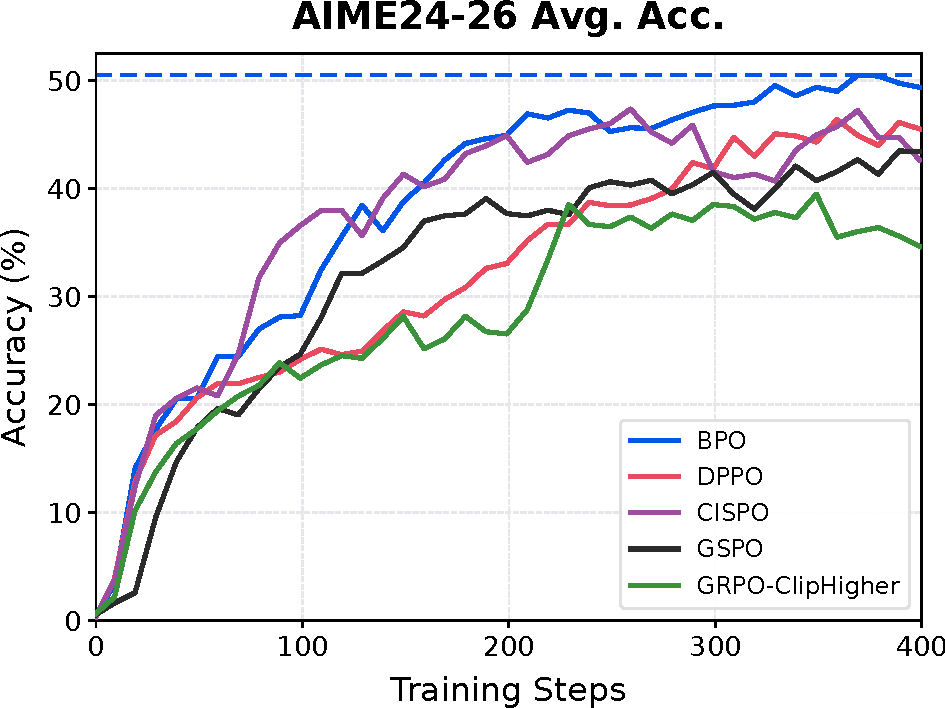
\includegraphics[width=0.8\linewidth]{figure/bpo_30b_aime_avg.pdf}
\caption{在Qwen3-30B-A3B-Base上的训练过程中，评估不同方法的准确率，包括BPO与GRPO-ClipHigher、GSPO、CISPO和DPPO的对比。所有方法均在DAPO-Math-17k的英文子集上训练400个训练步骤，实验设置相同，仅策略损失不同。每个批量滚动包含256个提示，每个提示生成16个响应，最大响应长度为16384 token。一个训练步骤包含一次滚动批量后接八次优化器更新。曲线显示AIME24--26的平均Avg@32准确率，每道题采样32个响应以估计Pass@1。水平虚线标记了BPO达到的峰值平均准确率。}
\label{fig:mainaime}
\end{figure}

组相对策略最优化（GRPO）及其变体在强化学习视觉推理（RLVR）中被广泛使用~\cite{shao2024deepseekmath,yu2026dapo,liu2025understanding,zheng2025gspo,chen2025minimax,zhang2026design,qi2026rethinking,liu2026prorl}。GRPO 为每个提示词采样多个响应，并通过在组内对奖励进行归一化来计算优势。在结果监督下，响应中的所有 token 共享相同的优势。GRPO 在 PPO 风格的裁剪代理目标中使用这些优势，结合 token 级别的重要性采样比率~\cite{schulman2017proximal}。该公式及其变体避免了训练价值模型，支持大规模推理模型训练~\cite{guo2025deepseek,yang2025qwen3,abdin2025phi,chen2025minimax,blakeman2025nvidia,blakeman2026nemotron,team2025every}。  

我们从策略镜像下降（Policy Mirror Descent, PMD）~\cite{lan2023policy,xiao2022convergence} 开始。PMD 使用动作值和散度惩罚来更新策略。然而，直接将此更新应用于语言生成需要在中间状态的值估计。一种常见方法是训练一个分离的价值模型，这会增加内存和计算成本~\cite{shao2024deepseekmath}。学成的价值估计在推理任务上也可能不准确~\cite{pmlr-v267-kazemnejad25a}。我们寻求对PMD的重新表述，使其在无需训练价值模型的情况下恢复相同的策略更新。

我们引入了贝尔曼策略最优化（BPO），这是一种从PMD推导出的无评论员策略最优化方法。我们的推导基于先前的工作，该工作使用策略似然比对奖励和价值进行重参数化~\cite{rafailov2023direct,zeng2024token,rafailovr,kang2026vimpo}。对于具有终端奖励的自回归生成，贝尔曼方程将每个token的优势表示为连续状态下的价值函数之差。这些差值沿着响应展开，最终仅留下终端奖励和初始价值。我们将这一恒等式与PMD最优性条件相结合，推导出一个轨迹级目标。  
初始价值是提示的期望奖励，可通过对采样响应进行估计。因此，这种重构避免了在中间状态估计价值或优势。  
我们证明了该目标与原始PMD目标在滚动策略可达的状态上具有相同的唯一最优解。 

随后，我们通过一系列近似推导出实际的 BPO 损失。我们使用为每个提示采样响应的平均奖励来估计初始值。我们近似轨迹级别的目标梯度，并用二元近似~\cite{qi2026rethinking} 替换完整的 KL 散度。所得梯度包含由回滚和当前 token 概率决定的不匹配修正权重。我们对该权重应用加性平滑以保证数值稳定性。在实际的 BPO 损失中，该权重取代了 GRPO 中使用的重要性采样比率。 

我们在基于 DAPO-Math-17k 训练的 Qwen3-30B-A3B-Base 上评估 BPO。  
在相同的实验设置下，我们与 GRPO-ClipHigher~\cite{shao2024deepseekmath,yu2026dapo}、GSPO~\cite{zheng2025gspo}、CISPO~\cite{chen2025minimax} 和 DPPO~\cite{qi2026rethinking} 进行对比。  
如图~\ref{fig:mainaime} 所示，BPO 在 AIME 2024--2026~\cite{aimeproblems} 上达到了 $50.5\%$ 的峰值平均准确率。  
相较于这四种基准方法，其提升分别为 $11.0$、$7.0$、$3.1$ 和 $4.1$ 个百分点。

我们的主要贡献是：

\begin{itemize}
\item 我们推导出一种无评论员、基于轨迹的PMD重表述方法，用于自回归生成中的终端奖励，避免在中间状态进行价值或优势估计。我们证明了该重表述与原始PMD目标在滚动策略可达状态下具有相同的唯一最优解。

\item 我们通过基于分组的估计和梯度近似，从这一重构形式中推导出实际的BPO损失。该损失用由互补token概率的平滑比给出的偏差校正权重，取代了GRPO的重要度采样比率。

\item 我们在数学推理基准上使用 Qwen3-30B-A3B-Base 评估 BPO。BPO 在 AIME 2024--2026 上达到峰值平均准确率为 $50.5\%$，相较于 GRPO-ClipHigher、GSPO、CISPO 和 DPPO 提升了 $3.1$ --$11.0$ 个百分点。

\end{itemize}

\FloatBarrier

\section{初步研究}\label{sec:prel1}

\subsection{符号标记}\label{sec:prel2}  
令 $\mathcal{V}$ 表示词表。  
令 $x$ 表示提示，令 $y=(y_1,\ldots,y_T)$ 表示响应。  
$x$ 与 $y$ 均为 $\mathcal{V}$ 上的 token 序列。  
在响应 $y$ 中，$y_t$ 是第 $t$ 个 token，且长度 $T$ 在不同响应中可能有所不同。  
我们还用 $|y|$ 来表示其长度。

对于 $1\leq t\leq u\leq T$ ，令 $y_{t:u}=(y_t,\ldots,y_u)$ 表示 $y$ 从位置 $t$ 到 $u$ 的子序列。我们记作 $y_{<t} = y_{1:t-1}$ ，$y_{\leq t} = y_{1:t}$ ，以及 $y_{\geq t} = y_{t:T}$ 。   

对于任意的 token 序列 $z_1,\ldots,z_k$ ，$(z_1,\ldots,z_k)$ 表示它们的拼接。例如，$(x,y_{<t})$ 表示提示 $x$ 后跟响应子序列 $y_{<t}$ 。 
对于参数为 token 序列的函数，当不会产生分歧时，我们用 $f(z_1,\ldots,z_k)$ 作为 $f((z_1,\ldots,z_k))$ 的简写形式。 

\subsection{RLVR作为一种周期性马尔可夫决策过程}
针对大模型（LLMs）的可验证奖励强化学习（RLVR）可被表述为一个有限时域的周期性马尔可夫决策过程（MDP）。 

令 $D$ 表示一个提示集，令 $\calD$ 表示在 $D$ 上的提示分布。  
为简化起见，我们假设 $\calD$ 在 $D$ 上是均匀分布的。该分析可直接推广到更一般的提示分布。

\paragraph{状态和转移。}
对于提示 $x\in D$，初始状态 $s_1$ 定义为序列 $x$ 本身。  
在步骤 $t>1$，状态 $s_t$ 将提示 $x$ 和生成的前缀 $y_{<t}$ 连结：  
$
    s_t = (x,y_{<t}).
$   
该转移是确定性的：将 token $y_t$ 添加到 $s_t=(x,y_{<t})$ 会得到下一个状态 $s_{t+1}=(x,y_{\leq t})$。  

\paragraph{政策与完成分布。}
令 $\Delta(\mathcal{V}) = \dr{p: \mathcal{V}\rightarrow[0,1]| \sum_{v\in\mathcal{V}}p(v)=1}$ 表示 $\mathcal{V}$ 上的概率分布的集合。  
随机性策略是一个映射 $\tpi:\calS \rightarrow \Delta(\mathcal{V})$。特别地，$\tpi(\cdot | x,y_{<t})\in\Delta(\mathcal{V})$ 表示位置 $t$ 处的下一个 token 分布。  
策略空间记为 $\policyspace = \Delta(\mathcal{V})^{\calS}$。  
对于任意策略 $\pi$，令 $\Pi_{\pi} \subseteq \Pi$ 表示相对于 $\pi$ 绝对连续的策略集合。

对于任意策略 $\tpi\in \policyspace$ 和状态 $s_t\in \calS$，我们用 $\mathbb{P}_{\pi}(\cdot | s_t)$ 表示由 $\tpi$ 诱导的完成分布，即 $\mathbb{P}_{\pi}(y_{\geq t}| s_t) = \prod_{u=t}^{|y|}\pi(y_u|s_u)$，其中 $y_{\geq t} = y_{t:|y|}$ 如第~\ref{sec:prel2} 节所述。 

在步骤 $t$  的动作是生成回复中的第 $t$ 个 token $y_t$ ，并从策略 $\tpi(\cdot | x, y_{<t})$ 中采样得到。  
实际上，$\pi$ 由一个自回归大语言模型参数化。  
当生成结束符 token（EOS）或达到回复长度限制 $T_{\max}$ 时，回复 $y = (y_1, \dots, y_T)$ 便终止。 

\paragraph{奖励与目标。}
一个确定性验证器 $R$ 会分配最终奖励。  
为不失一般性，我们假设对任意提示-响应对 $(x, y)$ ，均有 $|R(x, y)| \leq 1$ 。   

策略目标是  
\eql{\label{eq:J}}{
    \calJ(\pi)
    =
    \mathbb{E}_{x\sim \mathcal{D}, y\sim \cpi(\cdot| x)}
    \left[
    R(x,y)
    \right].
}

\subsection{群体相对策略最优化}
在实际的 RLVR 中，响应由 rollout 策略 $\mu$ 生成，而策略最优化则在当前策略 $\pi$ 上执行。  
rollout 生成与训练步骤之间的策略更新，以及 rollout 引擎与训练引擎之间的数值差异，可能导致这两个策略不一致~\cite{zheng2025stabilizing,qi2025defeating,qi2026rethinking,yao2026rethinking,yao2025rollout}。  
组相对策略最优化（Group-Relative Policy Optimization, GRPO）~\cite{shao2024deepseekmath} 是一种无需评论员（critic-free）、类 PPO 的策略最优化方法~\cite{schulman2017proximal}。  
对于每个提示 $x \sim \calD$ ，GRPO 独立地从 $\cmu(\cdot | x)$ 中采样一组 $G$ 个响应 $\dr{y^i}_{i=1}^{G}$ 。  
令 $R_i = R(x, y^i)$ 表示响应 $y^i$ 的奖励。  
GRPO 为每个响应分配组规范化的优势（group-normalized advantage）  
\eql{\label{eq:adv}}{
    \adv^i = \frac{R_i - \texttt{mean}\prb{\{R_j\}_{j=1}^{G}}}{\texttt{std}\prb{\{R_j\}_{j=1}^{G}}}.
}

GRPO 在 token 级别的重要性比率上应用了类似 PPO 的裁剪。  
对于响应 $y^i$ 中的第 $t$ 个 token，其每个 token 的损失定义为  
\eql{\label{eq:grpoloss}}{
    \calL_{i,t}^{\mathrm{GRPO}}(\pi) = -\min\dr{r_t^i\adv^i,\; \mathrm{clip}\pr{r_t^i, 1-\eps_{\mathrm{low}}, 1+\eps_{\mathrm{high}}}\adv^i},
}  
其中 $r_t^i$ 是定义为  
\eql{\label{eq:isratio}}{
    r_t^i = \frac{\pi(y_t^i | s_t^i)}{\mu(y_t^i | s_t^i)}.
}

以下每个 token 的损失与~\eqref{eq:grpoloss} 具有相同的梯度，因此在基于梯度的训练中是等价的：  
\eql{\label{eq:grpoloss-log}}{
    \widetilde{\calL}_{i,t}^{\mathrm{GRPO}}(\pi) = -\adv^i M_t^i \texttt{sg}\pr{r_t^i}\log\pi(y_t^i | s_t^i),
}  
其中，裁剪掩码 $M_t^i$ 定义为
\eql{\label{eq:maskgrpo1}}{
    M_t^i = \left\{\begin{array}{ll} 0, & \adv^i > 0 \text{ and } r_t^i > 1+\eps_{\mathrm{high}}, \\ 0, & \adv^i < 0 \text{ and } r_t^i < 1-\eps_{\mathrm{low}}, \\ 1, & \text{otherwise.} \end{array}\right.
}

\subsection{带有终局奖励的贝尔曼方程}\label{sec:BellmanEquations1}  
我们接下来介绍第~\ref{sec:prel1}节中描述的终局奖励情景下的价值函数和贝尔曼方程~\cite{sutton1998reinforcement}。  
对于一个固定的策略 $\tpi$ 和状态 $s_t = (x, y_{<t})$，定义价值函数为在策略 $\tpi$ 下给定状态 $s_t$ 时的期望奖励，即，  
\eql{\label{eq:V1}}{
    V^\tpi(s_t)
    =
    \Eb_{z \sim \cpi(\cdot|s_t)}\left[R(x,(y_{<t}, z)) \right],
}  
其中期望是针对在策略 $\tpi$ 下给定状态 $s_t = (x, y_{<t})$ 的所有完成情况计算的。  
因此，初始值 $V^{\tpi}(s_1) = V^{\tpi}(x)$ 是提示 $x$ 在策略 $\pi$ 下的期望奖励。  

由于中间奖励为零，对于非终止状态 $s_t$ ，动作价值函数定义为
\eql{\label{eq:Q2}}{
    Q^\tpi(s_t,y_t)
    =
    \mathbb{E}_{s'\sim \mathbb{P}(\cdot| s_t,y_t)}
    \left[V^\tpi(s')\right]= V^{\tpi}(s_{t+1}),
}
其中 $s_{t+1} = (s_t, y_t)$ ，第二个等式由第~\ref{sec:prel1} 节中描述的确定性转移得出。

对于非终止状态 $s_t$ ，优势函数定义为  
\eql{\label{eq:A1}}{
    A^\tpi(s_t,y_t) = Q^\tpi(s_t,y_t) - V^\tpi(s_t).
}  
优势函数 $A^\tpi(s_t,y_t)$ 衡量了在状态 $s_t$ 采取当前动作 $y_t$ 相对于策略 $\tpi(\cdot | s_t)$ 下的期望动作值的有利程度。  
由~\eqref{eq:V1} 和~\eqref{eq:A1} 可得  
\eql{\label{eq:avgA1}}{
    \sum_{y_t \in \mathcal{V}} \tpi(y_t | s_t) A^{\tpi}(s_t, y_t) = 0.  
} 

对于任意非终止状态 $s_t$ ，贝尔曼方程为
\eq{
    V^\tpi(s_t)
    =
    \sum_{y_t'\in \mathcal{V}} \tpi(y_t'| s_t) Q^\tpi(s_t,y_t')
    =
    \sum_{s'=(s_t,y_t'): y_t'\in \mathcal{V}} \tpi(y_t' | s_t) V^{\tpi}(s').
}
对于完整响应 $y$ ，终止状态为 $s_{|y|+1} = (x, y)$ 。终止条件为
\eq{
    V^{\tpi}(s_{|y| + 1}) = R(x,y).
}

\subsection{策略镜面下降}\label{sec:PMD} 
令 $\calS$ 表示状态空间，令 $\mathcal{V}$ 表示词表，如第~\ref{sec:prel1} 节所述。  
给定一个实值函数 $f: \mathcal{S} \x \mathcal{V} \rightarrow \Real$ ，策略镜面下降（PMD）~\cite{geist2019theory,lan2023policy,xiao2022convergence,tomar2020mirror} 为每个状态 $s \in \calS$ 求解如下最优化问题：
\eql{\label{eq:PMD}}{
    \max_{\pi(\cdot | s)\in \Delta(\mathcal{V})} \quad \Eb_{y\sim \pi(\cdot| s)}\br{f(s, y)} - \frac{1}{\eta} {\KL{\pi(\cdot| s)}{\mu(\cdot | s)}},                            
}
其中 $\mu$ 为行为策略（回放策略），$\eta > 0$ 为步长。 

最优化问题~\eqref{eq:PMD} 有唯一解
\eql{\label{eq:piexpw}}{
    \pi^+_{\mu, f}(y|s) = \frac{\mu(y|s)\exp\pr{\eta f(s, y)}}{Z_{\mu, f}(s) },
}
其中，配分函数为
\eq{
    Z_{\mu, f}(s) = \Eb_{y'\sim \mu(\cdot|s)} \exp\pr{\eta f(s, y')}.  
}

\subsection{二元KL散度}\label{sec:binary_kl}
设 $\pi, \mu \in \Pi$ 为定义在 $\mathcal{V}$ 上的两个策略。  
对于固定状态 $s$ ，它们的 KL 散度为  
\eq{
    \KL{\pi(\cdot|s)}{\mu(\cdot|s)}=
    \sum_{y\in\mathcal{V}}
    \pi(y | s)
    \log
    \frac{\pi(y | s)}{\mu(y | s)}.
}  
计算完整的 KL 散度需要整个词表的 Logit，计算开销较大。

引入的二值KL散度~\cite{qi2026rethinking} 近似了完整的KL散度。  
对于给定的动作 $y\in\mathcal{V}$ ，它将动作空间划分为 $\dr{y}$ 及其补集 $\mathcal{V}\setminus\dr{y}$ 。  
这诱导出以下伯努利分布：
\eq{
    \pi^{\mathrm{bin}}_y(\cdot| s)
    = \pr{\pi(y| s), 1 - \pi(y| s)},
    \quad
    \mu^{\mathrm{bin}}_y(\cdot| s)
    = \pr{\mu(y| s), 1 - \mu(y| s)}.
}
我们将与动作 $y$ 相关的二值KL散度定义为
\eql{\label{eq:binary_kl}}{
    &\quad D^{\mathrm{bin}}_{\mathrm{KL}}
    \pr{\pi(\cdot| s)\,\Vert\,\mu(\cdot| s); y}=
    D_{\mathrm{KL}}
    \pr{\pi^{\mathrm{bin}}_y(\cdot| s) \,\Vert\, \mu^{\mathrm{bin}}_y(\cdot| s)}
    \\
    &= \pi(y | s)\log\frac{\pi(y | s)}{\mu(y | s)} + \pr{1-\pi(y | s)}\log\frac{1-\pi(y | s)}{1-\mu(y | s)}.
}
如~\cite{qi2026rethinking} 所示，二值KL散度为KL散度提供了一个下界，即
\eq{
    0 \leq D^{\mathrm{bin}}_{\mathrm{KL}}\pr{\pi(\cdot| s) \,\Vert\, \mu(\cdot| s); y}
    \leq D_{\mathrm{KL}}\pr{\pi(\cdot| s) \,\Vert\, \mu(\cdot| s)}, \quad \forall y \in \mathcal{V}.  
} 

\section{贝尔曼策略最优化}
我们首先定义BPO损失，然后从PMD推导出它。

\paragraph{BPO损失定义。}
对于每个提示 $x\sim\calD$，我们独立地从一组 $G$ 个回复 $\dr{y^i}_{i=1}^G$ 中进行采样。  
对于回复 $y^i$ 的第 $t$ 个 token，BPO 损失为
\eql{\label{eq:bpoloss1}}{
    \calL^{\text{BPO}}(\pi) = - 
    \adv^i M^i_t\min\dr{\texttt{sg}\pr{\wt^i_{t}}, C} \log\pi(y^i_t| x, y^i_{<t}),  
}  
其中 $\adv^i$ 表示在组 $\dr{y^i}_{i=1}^G$ 中回复 $y^i$ 的优势，定义见~\eqref{eq:adv}，而项 $\wt^i_t$、$C$ 和 $M^i_t$ 定义如下：
\begin{itemize}
    \item $\wt^i_t$ 是响应 $y^i$ 中第 $t$ 个 token 的不匹配纠正权重，定义为  
    \eql{\label{eq:wti1}}{
        \wt^i_t = \frac{1 + \eps - \mu(y^i_t|x, y^i_{<t})}{1 + \eps - \pi(y^i_t|x, y^i_{<t})},  
    }

    \item 常数 $C$ 将 $\wt^i_t$ 限制以稳定训练。掩码 $M_t^i$ 遵循~\eqref{eq:maskgrpo1} 中的 GRPO 截断规则，其中权重 $\wt_t^i$ 取代了重要性采样比率： 
    \eq{
        M^i_t = 
        \left\{
        \begin{array}{ll}
            0, & \adv^i > 0 \text{ and } \wt^i_t > 1 + \eps_{\text{high}} \\
            0, & \adv^i < 0 \text{ and } \wt^i_t < 1 - \eps_{\text{low}} \\
            1, & \text{otherwise.}
        \end{array}
        \right.
    }
\end{itemize}
每个 token 的 BPO 损失保留了~\eqref{eq:grpoloss-log} 中的 GRPO 形式，并将重要性采样比率 $r_t^i$ 替换为截断的不匹配修正权重 $\min\dr{\stopgrad\pr{\wt_t^i}, C}$。

\paragraph{BPO目标的推导。} 
我们通过三个步骤推导出BPO目标~\eqref{eq:bpoloss1}：
\begin{itemize}
    \item 步骤 1（起点，~\eqref{eq:PMDadv1}）：我们使用 $f(s, y) = A^{\mu}(s, y)$ 实例化 PMD，其中 $A^{\mu}(s, y)$ 为第~\ref{sec:BellmanEquations1} 节中引入的优势函数。
    \item 步骤 2（无评论员的 PMD，第~\ref{sec:criticfreePMD}~节）：我们推导出一个无评论员的目标函数，其最优解与基于优势的 PMD 相同。这避免了在各个状态上估计 $A^\mu(s,y)$。  
    \item 步骤 3（实际近似，第~\ref{sec:binaryKL1} 节）：我们对步骤~2 中的无评论员 PDM 目标进行近似，以获得 BPO 目标~\eqref{eq:bpoloss1}。  
\end{itemize}

\paragraph{起点：基于优势的项目管理方法（PMD）。}
我们首先在~\eqref{eq:PMD} 中实例化通用的 PMD 目标，采用第~\ref{sec:BellmanEquations1} 节中终端奖励 MDP 的滚动策略优势 $A^{\mu}(s, y)$，即  
$
    f(s,y)=A^\mu(s,y).  
$  
经典 PDM 通常使用动作价值函数 $Q^\mu(s_t, y_t)$ ~\cite{geist2019theory,lan2023policy,xiao2022convergence,tomar2020mirror} 进行表述。使用 $A^\mu$ 可得到相同的更新，因为  
$
    Q^\mu(s_t, y_t)=A^\mu(s_t, y_t)+V^\mu(s_t),
$  
且项 $V^\mu(s_t)$ 与动作 $y_t$ 无关。 

基于优势的PMD为每个状态 $s_t = (x, y_{<t})$ 求解如下问题：
\eql{\label{eq:PMDadv1}}{
    \max_{\pi(\cdot | s_t)\in \Delta(\mathcal{V})} \quad \Eb_{y_t\sim \pi(\cdot| s_t)}\br{A^{\mu}(s_t, y_t)} - \frac{1}{\eta} {\KL{\pi(\cdot| s_t)}{\mu(\cdot | s_t)}}.                       
} 
如第~\ref{sec:PMD} 节所述，优化问题~\eqref{eq:PMDadv1} 具有唯一解 $\pi^+$ ，在每个状态 $s_t = (x, y_{<t})$ 处由下式给出
\eql{\label{eq:piexpwadv1}}{
    \pi^+(y_t|s_t) = \frac{\mu(y_t|s_t)\exp\pr{\eta A^{\mu}(s_t, y_t)}}{Z_{\mu}(s_t) },
}
其中，配分函数为
\eq{
    Z_{\mu}(s_t) = \Eb_{y'_t\sim \mu(\cdot|s_t)} \exp\pr{\eta A^{\mu}(s_t, y'_t)}.
}
此处，我们使用 $\pi^+$  和 $Z_{\mu}$  分别作为 $\pi^+_{\mu, A^{\mu}}$  和 $Z_{\mu, A^{\mu}}$ 的缩写。  

\subsection{无评论员的策略镜像下降重构}\label{sec:criticfreePMD}
直接实现更新~\eqref{eq:PMDadv1} 需要在每个访问的中间状态估计 $A^\mu(s_t,y_t)$。  
这通常需要一个学成的评论员或代价高昂的条件回放。  
我们通过将奖励和价值表示为策略似然比与贝尔曼方程，推导出无评论员的重表述形式~\eqref{eq:delta2}。这遵循了先前关于直接对齐的工作~\cite{rafailov2023direct,zeng2024token,rafailovr,kang2026vimpo}。 

\paragraph{无评论员的PMD重构}
令 $\mu$ 表示滚动策略。  
我们为每个提示 $x\in D$ 分配一个固定的正权重 $\phi(x)$。  
我们将在第~\ref{sec:binaryKL1} 节中指定该权重，以获得实际的 BPO 损失。  
我们考虑以下无评论员目标：  
\eql{\label{eq:delta2}}{
    \min_{\pi\in\Pi_\mu}
    \calL(\pi) = 
    \Eb_{x\sim \calD, y\sim\cmu(\cdot|x)}\br{\phi(x) \cdot \frac{\delta(x,y;\pi,\mu)^2}{2 \eta             }},   
}  
其中轨迹级残差 $\delta(x, y; \pi, \mu)$ 定义为  
\eql{\label{eq:deltadef1}}{
    \delta(x, y; \pi, \mu) = \eta \prb{R(x, y) - V^{\mu}(x)} - \sum_{t=1}^{|y|} \prB{\log\frac{\pi(y_t | s_t)}{\mu(y_t | s_t)} + \KL{\mu(\cdot | s_t)}{\pi(\cdot | s_t)}}.   
}

重述公式~\eqref{eq:delta2} 不依赖于中间状态的价值函数。相反，它仅需要终端奖励 $R(x,y)$ 和初始价值函数 $V^\mu(x)$ 。  
终端奖励 $R(x,y)$ 由验证器直接提供，而  
$
    V^\mu(x) = \Eb_{y\sim\cmu(\cdot|x)}\br{R(x,y)}
$ 
是提示 $x$ 在滚动策略 $\mu$ 下的期望奖励。  
我们可从滚动数据中估计该期望。

\paragraph{与PMD等效。}
定理~\ref{thm:delta2} 表明，无评论员目标~\eqref{eq:delta2} 和 PMD~\eqref{eq:PMDadv1} 具有相同的唯一最优解。  
该等价性对任意正权重函数 $\phi$ 均成立。  
我们在推导实际的 BPO 损失~\eqref{eq:bpoloss1} 时，于第~\ref{sec:binaryKL1} 节中指定了 $\phi$。

\begin{theorem}\label{thm:delta2}
    令策略 $\pi^+$ 在~\eqref{eq:piexpwadv1} 中表示 PDM 问题~\eqref{eq:PMDadv1} 的最优解。  
令 $\phi: D\rightarrow\Real_+$ 为提示集 $D$ 上的任意正权重函数。  
对于任意提示 $x \in D$ ，我们求解优化问题~\eqref{eq:delta2}。  
然后，该优化问题存在唯一的最优解 $\hat{\pi}^+$，其等于 $\pi^+$。  
此处的唯一性与等价性是指：  
任何求解~\eqref{eq:delta2} 的策略 $\hat{\pi}^+\in \Pi_{\mu}$ 对每个提示 $x\in D$ 均诱导出与 $\pi^+$ 相同的补全分布，即 $\cpx{\hat{\pi}^+}(\cdot|x) = \cpx{\pi^+}(\cdot|x)$。          
\end{theorem}

我们现在推导目标~\eqref{eq:delta2} 并概述定理~\ref{thm:delta2} 的证明。 

\paragraph{充分性推导与证明。}
我们首先解释如何从基于优势的原始PMD~\eqref{eq:PMDadv1}推导出无评论员的目标~\eqref{eq:delta2}，并证明PMD解~$\pi^+$ 最小化重构后的目标~\eqref{eq:delta2}。

\vspace{0.2cm}
\noindent$\bullet$ ~步骤~1：我们将~\eqref{eq:piexpwadv1} 重写为 PMD 最优性条件，并消去依赖于状态的配分函数 $Z_{\mu}(s_t)$ 。  
对于任意提示 $x$ 、响应 $y$ 和满足 $1\leq t \leq |y|$ 的步数 $t$ ，我们可以将~\eqref{eq:piexpwadv1} 重写为  
\eql{\label{eq:PMD2}}{
    \log\pi^+(y_t | s_t) - \log\mu(y_t | s_t) - \eta A^{\mu}(s_t, y_t) + \log Z_{\mu}(s_t) = 0.  
} 
对 $y_t \sim \mu(\cdot | s_t)$ 取期望并利用~\eqref{eq:avgA1} ，可得  
\eql{\label{eq:logparti1}}{
    \log Z_{\mu}(s_t) = \KL{\mu(\cdot | s_t)}{\pi^+(\cdot | s_t)} + \eta \sum_{y_t\in \mathcal{V}} \mu(y_t | s_t) A^{\mu}(s_t, y_t) = \KL{\mu(\cdot | s_t)}{\pi^+(\cdot | s_t)}.      
} 
接着，将~\eqref{eq:logparti1} 代入~\eqref{eq:PMD2} ，得到  
\eql{\label{eq:PMDKL1}}{
    \log\pi^+(y_t | s_t) - \log\mu(y_t | s_t) - \eta A^{\mu}(s_t, y_t) + \KL{\mu(\cdot | s_t)}{\pi^+(\cdot | s_t)}= 0.  
}  

\noindent$\bullet$ ~步骤2：接下来，我们用最终奖励表示累积的token级优势。根据贝尔曼方程，将~\eqref{eq:Q2}代入~\eqref{eq:A1}得
\eq{
    A^{\mu}(s_t,y_t)=V^{\mu}(s_{t+1}) - V^{\mu}(s_t).
}
对轨迹求和得
\eql{\label{eq:sumA1}}{
    \sum_{t=1}^{|y|} A^{\mu}(s_t, y_t) = V^{\mu}(s_{|y|+1}) - V^{\mu}(s_1) = R(x, y) - V^{\mu}(x).   
} 

\noindent$\bullet$ ~步骤~3：对于任意的提示-响应对 $(x, y)$ ，对轨迹求和~\eqref{eq:PMDKL1} 并使用~\eqref{eq:sumA1} 得到  
\eq{
    \sum_{t=1}^{|y|} \pr{\log\pi^+(y_t | s_t) - \log\mu(y_t | s_t) + \KL{\mu(\cdot | s_t)}{\pi^+(\cdot | s_t)}}= \eta \pr{R(x, y) - V^{\mu}(x)},     
}
即，  
\eql{\label{eq:sumdelta2}}{
    \delta(x, y; \pi^+, \mu) = 0. 
}
在滚动分布下最小化期望平方残差得到~\eqref{eq:delta2}。 

\paragraph{必要性证明概要。}
还需证明~\eqref{eq:delta2} 的每个最优解在 $\mu$ 下可达的所有状态上均与 $\pi^+$ 一致。  
定义 token 级残差：  
\eq{
    d_\pi(s_t, y_t) = \eta A^\mu(s_t,y_t) -
    \prB{\log\pi(y_t|s_t) - \log\mu(y_t|s_t) + \KL{\mu(\cdot|s_t)}{\pi(\cdot|s_t)}}.  
}  
对任意可行策略 $\pi$（使得上述量有限），其在 rollout 策略下的条件期望为零：  
\eq{
    \Eb_{y_t\sim\mu(\cdot|s_t)}\br{d_\pi(s_t,y_t)}= \eta\sum_{y_t\in\mathcal V}\mu(y_t|s_t)A^\mu(s_t,y_t) - \sum_{y_t\in\mathcal V}\mu(y_t|s_t)\log\frac{\pi(y_t|s_t)}{\mu(y_t|s_t)} - \KL{\mu(\cdot|s_t)}{\pi(\cdot|s_t)}= 0.  
}  
因此，累计 token 级残差在 rollout 策略 $\mu$ 下构成一个鞅。  
对任意~\eqref{eq:delta2} 的最优解，该鞅的终值等于轨迹级残差，且几乎必然为零。由于响应长度以 $T_{\max}$ 为界，鞅性质即推出每个部分和几乎必然为零，故每个 token 级残差均消失。  
完整证明见附录~\ref{sec:prfdelta2}。 

\subsection{实用近似}\label{sec:binaryKL1}

我们通过近似无评论员目标~\eqref{eq:delta2}，得到了实用的BPO损失~\eqref{eq:bpoloss1}。我们对平方残差目标进行线性化，并从分组回溯中估计初始值和与提示相关的缩放因子。然后，我们使用二元KL散度近似完整的逆向KL散度，并应用平滑、掩码和截断。 

对于响应 $y^i$，定义响应级别的损失 $\calL_i(\pi) = \phi(x)\delta(x,y^i;\pi,\mu)^2/(2\eta)$。  
其梯度可分解为 token 级别的贡献 $
    \na\calL_i(\pi)
    = \sum_{t=1}^{|y^i|} \na\calL_{i,t}(\pi).  
$。  
在本节中，$\na$ 表示相对于 $\pi$ 参数的梯度，同时保持 $\mu$ 固定。

\vspace{0.2cm}
\noindent$\bullet$ ~步骤~1：线性近似。  
我们对关于残差 $\delta$ 的方阵残差损失进行线性化，在 $\pi=\mu$ 处对其取值进行线性化。  
由于 $\delta(x,y^i;\mu,\mu) = \eta\pr{R(x,y^i)-V^\mu(x)}$ ，  
这将梯度中的残差因子 $\delta(x,y^i;\pi,\mu)/\eta$ 替换为 $R(x,y^i)-V^\mu(x)$ 。  
对于响应 $y^i$ 及其对应的状态 $s_t^i = (x, y_{<t}^i)$ ，每个 token 的梯度贡献近似为  
\eql{\label{eq:est1}}{
    \na \calL_{i,t}(\pi) 
    &= -\phi(x)\frac{\delta(x, y^i; \pi, \mu)}{\eta}\na\prB{\log\pi(y_t^i | s_t^i) + \KL{\mu(\cdot | s_t^i)}{\pi(\cdot | s_t^i)}} \\  
    &\approx -\phi(x)\prB{R(x, y^i) - V^\mu(x)}\na\prB{\log\pi(y_t^i | s_t^i) + \KL{\mu(\cdot | s_t^i)}{\pi(\cdot | s_t^i)}}.
}

\noindent$\bullet$ ~步骤2：基于分组的估计与规范化。  
初始价值函数 $V^\mu(x) = \Eb_{y\sim\cmu(\cdot | x)}\br{R(x, y)}$ 
具有无偏估计量 $\texttt{mean}\prb{\{R(x, y^j)\}_{j=1}^{G}}$ 。  
我们进一步选择 $\phi(x)$ 作为奖励标准差的倒数，即 $\phi(x) = \frac{1}{\sqrt{\text{Var}_{y\sim \cmu(\cdot|x)}(R(x, y))}}$ 。 我们用其经验对应项 $\phi(x) \approx \frac{1}{\texttt{std}\prb{\{R(x, y^i)\}_{i=1}^G}}$ 替换它。  
经过这些置换后，~\eqref{eq:est1} 变为
\eql{\label{eq:est2}}{
    \na \calL_{i,t}(\pi) \approx 
    - \adv^i \na\prB{\log\pi(y_t^i | s_t^i) + \KL{\mu(\cdot | s_t^i)}{\pi(\cdot | s_t^i)}}.
}

\noindent$\bullet$ ~步骤3：二值KL近似与加法平滑。  
在~\eqref{eq:est2} 中计算完整的逆向KL散度可能代价较高。  
因此，我们将~\eqref{eq:est2} 中的完整KL散度 $\KL{\mu(\cdot | s_t^i)}{\pi(\cdot | s_t^i)}$ 替换为如第~\ref{sec:binary_kl} 节所定义的二值KL散度 $D^{\mathrm{bin}}_{\mathrm{KL}}\pr{\mu(\cdot | s_t^i) \,\Vert\, \pi(\cdot | s_t^i); y_t^i}$。  
如附录~\ref{sec:proof-binary-kl-gradient} 所证明，以下恒等式成立  
\eql{\label{eq:binary-kl-gradient1}}{
    \na\prB{\log\pi(y_t^i | s_t^i) + D^{\mathrm{bin}}_{\mathrm{KL}}\pr{\mu(\cdot | s_t^i) \,\Vert\, \pi(\cdot | s_t^i); y_t^i}}={\frac{1 - \mu(y_t^i | s_t^i)}{1 - \pi(y_t^i | s_t^i)}}\na\log\pi(y_t^i | s_t^i).
}  
将~\eqref{eq:binary-kl-gradient1} 代入~\eqref{eq:est2} 得到  
\eql{\label{eq:est3}}{
    \na \calL_{i,t}(\pi) \approx  - \adv^i{\frac{1 - \mu(y_t^i | s_t^i)}{1 - \pi(y_t^i | s_t^i)}}\na \log\pi(y_t^i | s_t^i).
}  
当 $\pi(y_t^i | s_t^i)$ 接近1时，~\eqref{eq:est3} 中的乘子 $\frac{1 - \mu(y_t^i | s_t^i)}{1 - \pi(y_t^i | s_t^i)}$ 可能变得很大。为保证数值稳定性，我们采用~\eqref{eq:wti1} 中定义的加法平滑错配校正权重 $\wt_t^i$。   
最终的每个token梯度为  
\eql{\label{eq:est4}}{
    \na \calL_{i,t}(\pi) 
    \approx -\adv^i\wt_t^i\na\log\pi(y_t^i | s_t^i).
}

\noindent$\bullet$ ~步骤~4：掩码与裁剪。  
前面的步骤得到了近似的每个 token 的梯度方向 $-\adv^i\wt_t^i\na\log\pi(y_t^i | s_t^i).$ 

我们应用 GRPO 风格的裁剪掩码 $M_t^i$ 并将 $\wt_t^i$ 限制在 $C$ 。由此得到的 per-token BPO 损失梯度为
\eq{
    \na \calL_{i,t}^{\mathrm{BPO}}(\pi) = -\adv^i M_t^i\min\dr{{\wt_t^i}, C}\na \log\pi(y_t^i | s_t^i).  
}
这给出了 BPO 损失~\eqref{eq:bpoloss1}。

\section{实验}\label{sec:experiments}

\subsection{实验设置}
我们在数学推理任务中对 BPO 进行评估，使用 Qwen3-30B-A3B-Base~\cite{yang2025qwen3}。所有方法均在 DAPO-Math-17k~\cite{yu2026dapo} 的英文子集上进行训练。我们对比 BPO 与 GRPO-ClipHigher~\cite{shao2024deepseekmath,yu2026dapo}、GSPO~\cite{zheng2025gspo}、CISPO~\cite{chen2025minimax} 和 DPPO~\cite{qi2026rethinking}。通过仅改变策略损失（Policy Loss）而保持其他所有实验设置一致，进行受控比较。 

每个回溯批量包含 256 个提示，每个提示生成 16 个回复。产生的 4096 个回复被划分为 8 个小批量，每个小批量包含 512 个回复。一次训练步骤包含一个回溯批量及其对应的八个小型批量更新。我们对每种方法进行 400 次训练步骤的训练，相当于 3200 次优化器更新。最大回复长度为 16384 token。所有方法均使用回溯-路由重放（R3）~\cite{ma2025stabilizing}。BPO 使用 $\epsilon=0.1$ 和 $C=3.0$。这些超参数的消融实验结果见附录~\ref{sec:ablations}。更多细节见附录~\ref{sec:experimentdetails}。

我们在 AIME24、AIME25 和 AIME26~\cite{aimeproblems} 上进行评估。我们使用 Avg@32 估计 Pass@1：对每个问题采样 32 个回答，计算其正确性的平均值，然后在问题间取平均。平均准确率是三个基准得分的算术平均值。表~\ref{tab:mainaime} 报告了各方法在三个基准上平均准确率最高的检查点处的结果。 

\subsection{主要结果}
表~\ref{tab:mainaime} 显示，BPO 的平均准确率为 50.5\%，而 GRPO-ClipHigher 为 39.5\%，CISPO（最强基准）为 47.4\%，分别提升了 11.0 和 3.1 个百分点。BPO 在所有三个基准上均达到了最高准确率。

BPO 达到了最高的最终准确率（图~\ref{fig:mainaime}）。经过 400 次训练步骤后，其平均准确率为 49.4\%，而最强的基准方法 DPPO 在训练结束时的准确率为 45.5\%。

\begin{table}[htbp]
\centering
\caption{Qwen3-30B-A3B-Base 上的 AIME 平均得分@32（\%）。每一行报告在三个基准上平均准确率最高的检查点得分。每列中最佳结果以粗体显示。}
\label{tab:mainaime}
\small
\renewcommand{\arraystretch}{1.1}
\begin{tabular}{lcccc}
\hline
Method & AIME24 & AIME25 & AIME26 & Avg. \\
\hline
GRPO-ClipHigher & 45.6 & 34.8 & 38.0 & 39.5 \\
GSPO & 50.3 & 35.5 & 44.6 & 43.5 \\
CISPO & 52.7 & 39.0 & 50.4 & 47.4 \\
DPPO & 55.8 & 39.2 & 44.2 & 46.4 \\
BPO & \textbf{57.4} & \textbf{41.0} & \textbf{53.0} & \textbf{50.5} \\
\hline
\end{tabular}
\end{table}

\FloatBarrier

\section{结论}\label{sec:conclusion}
我们提出了贝尔曼策略最优化（BPO），这是一种从策略镜像下降（PMD）导出的无需评论员的强化学习视觉推理（RLVR）方法。利用贝尔曼方程，我们得到了一个轨迹级目标，该目标避免了对中间状态值的估计。我们证明了该目标与原始PMD目标在滚动策略可到达的状态上具有相同的唯一最优解。随后，通过近似推导出一种实用的token级损失，其中使用平滑化的不匹配修正权重替代重要性采样比率。在Qwen3-30B-A3B-Base上，BPO在AIME 2024--2026期间达到峰值平均准确率为$50.5\%$，优于GRPO-ClipHigher、GSPO、CISPO和DPPO $3.1$--$11.0$个百分点。在Qwen3-4B-Base上的消融实验表明，在一系列平滑和截断设置下，性能表现相似。

\section*{致谢}
我们感谢Sam、Lingfeng、Chris、Simon、Beibin、Yifan、Charlotte、Ziven、Robert、Yuzhen、Yingying、Xingxuan、Zhenwen、Feng、Kaiyu、Kevin、Chen、Chenchen、Ziran和Marcus的有益讨论。本文稿的语言编辑和校对使用了ChatGPT和Claude。代码调试则借助了Codex和Claude Code。  

\FloatBarrier

\bibliography{ref}

\begin{appendices}

\section{省略的证明}
\subsection{定理~\ref{thm:delta2} 的证明}\label{sec:prfdelta2}
充分性由~\eqref{eq:sumdelta2} 直接得出。  
还需证明必要性。  
在本节中，我们用 $\mathbb{I}_A$ 表示事件 $A$ 的指示函数。  

令 $\text{supp}\mu(\cdot|s)$ 表示在状态 $s$ 下，策略 $\mu$ 所赋予正概率的动作集合。  
令 $\text{supp}\cmu(\cdot|x)$ 表示在提示 $x$ 给定的情况下，策略 $\mu$ 所赋予正概率的响应集合。  
令 $\calS_x^\mu$ 表示从提示 $x$ 出发，在策略 $\mu$ 下以正概率可达的状态集合。

修复任意提示 $x\in D$。
对于任意状态-动作对 $(s,a)$，定义
\eq{
    d_\pi(s,a) = \eta A^\mu(s,a) - \prB{\log\pi(a|s) - \log\mu(a|s) + \KL{\mu(\cdot|s)}{\pi(\cdot|s)}}.
}
根据定义，
\eql{\label{eq:deltasumdt}}{
    \delta(x,y;\pi,\mu) = \sum_{t=1}^{|y|} d_\pi(s_t,y_t).
}
我们首先证明~\eqref{eq:delta2} 的极小点为零。
PM D 最优性条件~\eqref{eq:PMDKL1} 给出
\eq{
    d_{\pi^+}(s,a)=0.
}
指数形式更新~\eqref{eq:piexpwadv1} 保持了滚动策略的支持集，因此 $\pi^+\in\Pi_\mu$ 且
\eq{
    \delta(x,y;\pi^+,\mu)=0,
    \quad
    \forall y\in\text{supp}\cmu(\cdot|x).
}
因此，$\pi^+$ 对于~\eqref{eq:delta2} 是可行的，并达到目标值零。
由于目标函数非负，~\eqref{eq:delta2} 的最小值为零。

现在令 $\hat{\pi}^+\in\Pi_\mu$ 为 \eqref{eq:delta2} 的任意最优解。  
由于极小值为零且 $\phi(x) > 0$ ，我们有  
\eql{\label{eq:deltapizero1}}{
    \delta(x,Y;\hat{\pi}^+,\mu)=0,
    \quad
    Y\sim\cmu(\cdot|x)\text{-almost surely}.  
}  
由于目标值有限，对于每个状态 $s\in\calS_x^\mu$ ，  
$\KL{\mu(\cdot|s)}{\hat{\pi}^+(\cdot|s)} < \infty. $  
因此，对于任意 $s\in \calS_x^{\mu}$ ，$\mu(\cdot|s)$ 相对于 $\hat{\pi}^+(\cdot|s)$ 绝对连续。  
因此，以下所有量在 $\mu$ 下可达的状态上均为有限值。  

设 $\tau$ 为生成终止的时间：  
\eq{
    \tau= \inf\dr{t\geq 1: Y_t=\mathrm{EOS}} \wedge T_{\max}.
}
定义滤波
\eq{
    \calF_t= \sigma\pr{Y_1,\dots,Y_{t\wedge\tau}}, \quad 0\leq t\leq T_{\max}.   
}
对于 $1\leq t\leq T_{\max}$，定义
\eq{
    D_t = \mathbb{I}_{\dr{t\leq\tau}}d_{\hat{\pi}^+}(S_t,Y_t), \quad
    M_n = \sum_{t=1}^n D_t,
}
其中 $S_t=(x,Y_{<t})$ 在事件 $\dr{t\leq\tau}$ 上。

由于 $\mathbb{I}_{\dr{t\leq\tau}}$ 和 $S_t$ 是
$\calF_{t-1}$ -可测的，我们有
\eq{
    &\quad \Eb\br{D_t\mid\calF_{t-1}} \\
    &= \mathbb{I}_{\dr{t\leq\tau}}\sum_{a\in\mathcal V}\mu(a|S_t)d_{\hat{\pi}^+}(S_t,a)
    \\
    &= \mathbb{I}_{\dr{t\leq\tau}}\eta\sum_{a\in\mathcal V}\mu(a|S_t)A^\mu(S_t,a)
    \\
    &\quad
    - \mathbb{I}_{\dr{t\leq\tau}}\prB{\sum_{a\in\mathcal V}\mu(a|S_t)\log\frac{\hat{\pi}^+(a|S_t)}{\mu(a|S_t)}
    +
    \KL{\mu(\cdot|S_t)}{\hat{\pi}^+(\cdot|S_t)}}
    \\
    &=0,  
}
其中最后一个等式来自~\eqref{eq:avgA1}。 
因此，$\dr{M_n}_{n=0}^{T_{\max}}$ 是一个可积鞅。

由~\eqref{eq:deltasumdt} 和~\eqref{eq:deltapizero1}，
\eq{
    M_{T_{\max}} = \sum_{t=1}^{\tau} d_{\hat{\pi}^+}(S_t,Y_t) = \delta(x,Y;\hat{\pi}^+,\mu) = 0, \quad \text{$\cmu(\cdot|x)$-almost surely.}
}
因此，对于任意 $0\leq n\leq T_{\max}$ ，
\eq{
    M_n = \Eb\br{M_{T_{\max}} | \calF_n}= 0,
    \quad \text{$\cmu(\cdot|x)$-almost surely.}
}
由此可得，对于任意 $1\leq t\leq T_{\max}$ ，
\eq{
    D_t = M_t - M_{t-1} = 0 \quad \text{$\cmu(\cdot|x)$-almost surely.}
}
考虑任意状态 $s\in\calS_x^\mu$ 和任意动作
$a\in\text{supp}\mu(\cdot|s)$。
对于相应的步骤 $t$，事件 $\dr{S_t=s, Y_t=a}$ 在 $\cmu(\cdot|x)$ 下具有严格正的概率。
由于 $D_t=0$ 几乎必然成立，这表明
\eq{
    d_{\hat{\pi}^+}(s,a)=0.
}
结合 $d_{\pi^+}(s,a)=0$，我们得到
\eq{
    \log\frac{\hat{\pi}^+(a|s)}{\pi^+(a|s)} = \KL{\mu(\cdot|s)}{\pi^+(\cdot|s)} - \KL{\mu(\cdot|s)}{\hat{\pi}^+(\cdot|s)}.  
}
右边不依赖于 $a$。
因此，对每个 $s\in\calS_x^\mu$，存在常数 $c(s)>0$ 使得
\eq{
    \hat{\pi}^+(a|s) = c(s)\pi^+(a|s), \quad \forall a\in\text{supp}\mu(\cdot|s).
}
由于 $\hat{\pi}^+,\pi^+\in\Pi_\mu$，两个策略在 $\text{supp}\mu(\cdot|s)$ 外均赋予零概率。
因此，
\eq{
    1 = \sum_{a\in\text{supp}\mu(\cdot|s)}
    \hat{\pi}^+(a|s)
    = c(s)\sum_{a\in\text{supp}\mu(\cdot|s)}
    \pi^+(a|s)
    = c(s).  
}
故 $c(s)=1$，且
\eq{
    \hat{\pi}^+(\cdot|s) = \pi^+(\cdot|s), \quad \forall s\in\calS_x^\mu.
}
此外，由于 $\hat{\pi}^+,\pi^+\in\Pi_\mu$，$\pi^+$ 与 $\hat{\pi}^+$ 均在 $\text{supp}\cmu(\cdot|x)$ 外赋予零概率。
因此，
\eq{
    \cpx{\hat{\pi}^+}(\cdot|x) = \cpx{\pi^+}(\cdot|x).  
}
证明完成。
\hfill $\square$

\subsection{恒等式~(\ref{eq:binary-kl-gradient1}) 的证明}\label{sec:proof-binary-kl-gradient}
固定一个状态 $s$ 和一个动作 $y$ ，并令  
\eq{
    p = \pi(y | s),\quad q = \mu(y | s).
}  
与动作 $y$ 有关的二元 KL 散度为  
\eq{
    D^{\mathrm{bin}}_{\mathrm{KL}}\pr{\mu(\cdot | s) \,\Vert\, \pi(\cdot | s); y}= q\log\frac{q}{p} + (1 - q)\log\frac{1 - q}{1 - p}.
}  
对 $\pi$ 求导得  
\eq{
    \na D^{\mathrm{bin}}_{\mathrm{KL}}\pr{\mu(\cdot | s) \,\Vert\, \pi(\cdot | s); y}= -q\na\log p + \frac{1 - q}{1 - p}\na p.
}  
利用 $\na p = p\na\log p$ 这一事实，我们得到  
\eq{
    \na\prB{\log p + D^{\mathrm{bin}}_{\mathrm{KL}}\pr{\mu(\cdot | s) \,\Vert\, \pi(\cdot | s); y}}= (1 - q)\na\log p + \frac{(1 - q)p}{1 - p}\na\log p
    = \frac{1 - \mu(y | s)}{1 - \pi(y | s)}\na\log\pi(y | s),                 
}  
即  
\eq{
    \na\prB{\log\pi(y | s) + D^{\mathrm{bin}}_{\mathrm{KL}}\pr{\mu(\cdot | s) \,\Vert\, \pi(\cdot | s); y}}= \frac{1 - \mu(y | s)}{1 - \pi(y | s)}\na\log\pi(y | s).
}  
这证明了~\eqref{eq:binary-kl-gradient1}。  
\hfill $\square$

\section{实验细节}\label{sec:experimentdetails}

所有实验均采用 AdamW 优化器，学习率为 $10^{-6}$ ，$\beta_1=0.9$ ，$\beta_2=0.98$ ，权重衰减为 $0.1$ 。梯度裁剪阈值为 $1.0$ 。我们不使用 KL 惩罚，熵奖励系数为零。  
训练时的 rollout 采样温度为 $1.0$ ，top-$p=1.0$ ，并禁用 top-$k$ 过滤。优势值在每个响应组内按奖励标准差进行中心化和规范化，方法与 GRPO 一致。  
我们使用 \texttt{seq-mean-token-mean} 作为损失聚合方式。  
这些设置在各方法间共享。

我们在第~\ref{sec:experiments} 节的主要实验中使用 400 次训练步骤，而在附录~\ref{sec:ablations} 的消融实验中使用 1000 次。  
AIME 基准数据集可在 Hugging Face 上获取。\footnote{AIME24：\url{https://huggingface.co/datasets/math-ai/aime24}，AIME25：\url{https://huggingface.co/datasets/math-ai/aime25}，AIME26：\url{https://huggingface.co/datasets/math-ai/aime26}。} 我们每十批回溯（即训练步骤）进行一次评估。  
所有评估在温度 $1.0$ 和 top-$p=1.0$ 下使用每个问题 32 个回复，且禁用 top-$k$ 过滤。评估时每个模型使用的回复长度限制与训练时相同。

我们以Avg@32作为Pass@1的估计值。  
Avg.列和绘制的平均准确率是AIME24、AIME25和AIME26的Avg@32得分的算术平均值。

我们选择在三个基准上平均Avg@32值最高的检查点，若出现平局则选择较早的步骤。 

GRPO-ClipHigher 使用了来自 DAPO~\cite{yu2026dapo} 的非对称裁剪区间 $[0.8,1.28]$。CISPO 采用了重要性权重上限 $3.0$，遵循 DPPO~\cite{qi2026rethinking} 中稳定性实验所使用的配置。DPPO 使用了阈值为 $\delta=0.1$ 的二值总变差，遵循 TMax~\cite{ivison2026tmax}。GSPO 使用了裁剪区间 $[1-3\times10^{-3},1+5\times10^{-3}]$，遵循~\cite{khatri2026art} 中的消融结果。BPO 在主实验中使用了默认情景 $\epsilon=0.1$ 和 $C=3.0$。

\section{消融研究}\label{sec:ablations}
我们研究了在 Qwen3-4B-Base 上进行 1000 次训练步骤时，两个 BPO 超参数 $\eps$  和 $C$  的影响。  
此处，每个批量包含 128 个提示，每个提示对应 16 个回复。共 2048 个回复被划分为四个小批量，每个小批量为 512 个回复，最大回复长度为 8192 token。图中每一个训练步骤表示一次滚动生成批量及其对应的小批量更新。  
每次扫描仅改变一个超参数，其余设置保持不变。第~\ref{sec:epsilonablation}~节和第~\ref{sec:capablation}~节中的两次扫描均采用附录~\ref{sec:experimentdetails}~中的训练设置，并共享相同的 GRPO-ClipHigher 基准。

\subsection{对 $\epsilon$ 的敏感性 }\label{sec:epsilonablation}
我们固定 $C=3.0$ 并在 $\{0.05,0.1,0.2,0.3\}$ 范围内变化 $\epsilon$。图~\ref{fig:epsilonablation} 显示了训练曲线，表~\ref{tab:epsilonablation} 总结了结果。

\begin{figure}[htbp]
\centering
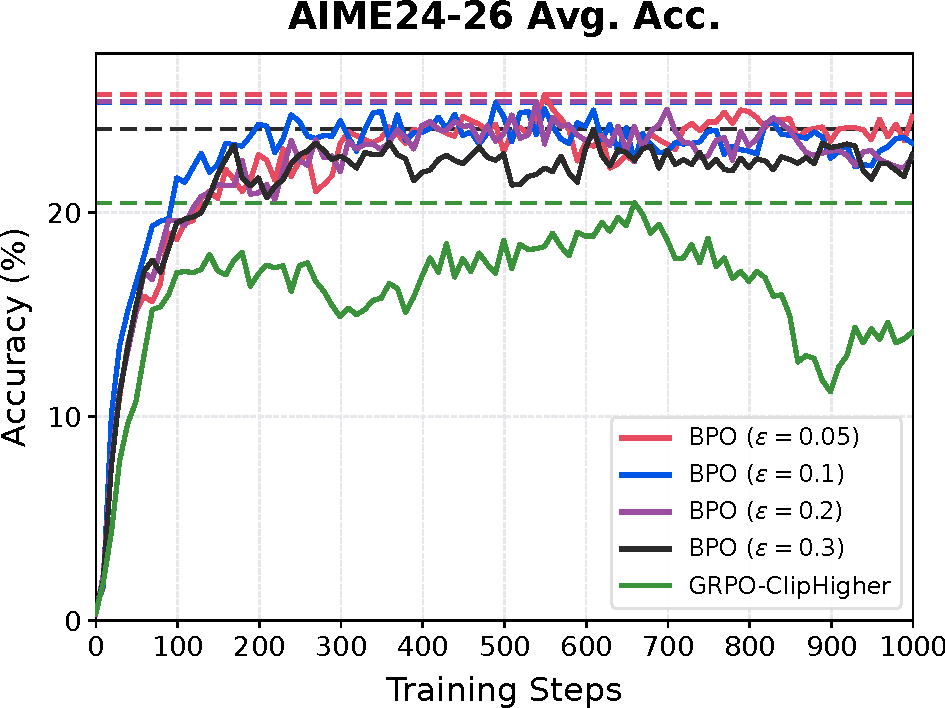
\includegraphics[width=0.8\linewidth]{figure/ab_bpo_4b_eps_aime_avg.pdf}
\caption{BPO的平滑参数$\epsilon$对Qwen3-4B-Base的影响，其中$C=3.0$。曲线展示了AIME24--26期间平均Avg@32的数值。虚线标记了每条曲线的峰值。}
\label{fig:epsilonablation}
\end{figure}

\begin{table}[htbp]
\centering
\caption{BPO 的平滑参数 $\epsilon$  的消融实验，使用 $C=3.0$ ，报告 AIME Avg@32 (\%)。每一行报告在三个基准上平均准确率最高的检查点的得分。每列中最佳结果加粗。}
\label{tab:epsilonablation}
\small
\renewcommand{\arraystretch}{1.1}
\begin{tabular}{lrrrr}
\hline
Method & AIME24 & AIME25 & AIME26 & Avg. \\
\hline
BPO ($\epsilon=0.05$) & \textbf{31.6} & 23.0 & 22.8 & \textbf{25.8} \\
BPO ($\epsilon=0.1$) & 27.6 & \textbf{26.8} & 21.8 & 25.4 \\
BPO ($\epsilon=0.2$) & 29.1 & 24.3 & \textbf{23.0} & 25.5 \\
BPO ($\epsilon=0.3$) & 26.4 & 25.5 & 20.4 & 24.1 \\
GRPO-ClipHigher & 22.1 & 22.8 & 16.6 & 20.5 \\
\hline
\end{tabular}
\end{table}

BPO 在 $\epsilon\in\{0.05,0.1,0.2\}$ 情景下的平均准确率均达到 25.4\%--25.8\%。在 $\epsilon=0.3$ 情景下，准确率为 24.1\%，仍比 GRPO-ClipHigher 高出 3.6 个百分点。BPO 对 $\epsilon$ 从 $0.05$ 到 $0.2$ 的变化表现出较低的敏感性，并在所有四个设置中均优于基准。

\FloatBarrier

\subsection{对 $C$ 的敏感性 }\label{sec:capablation}
我们固定 $\epsilon=0.1$ 并在 $\{2.0,3.0,4.0\}$ 范围内变化 $C$。图~\ref{fig:capablation} 显示了训练曲线，表~\ref{tab:capablation} 总结了结果。

\begin{figure}[htbp]
\centering
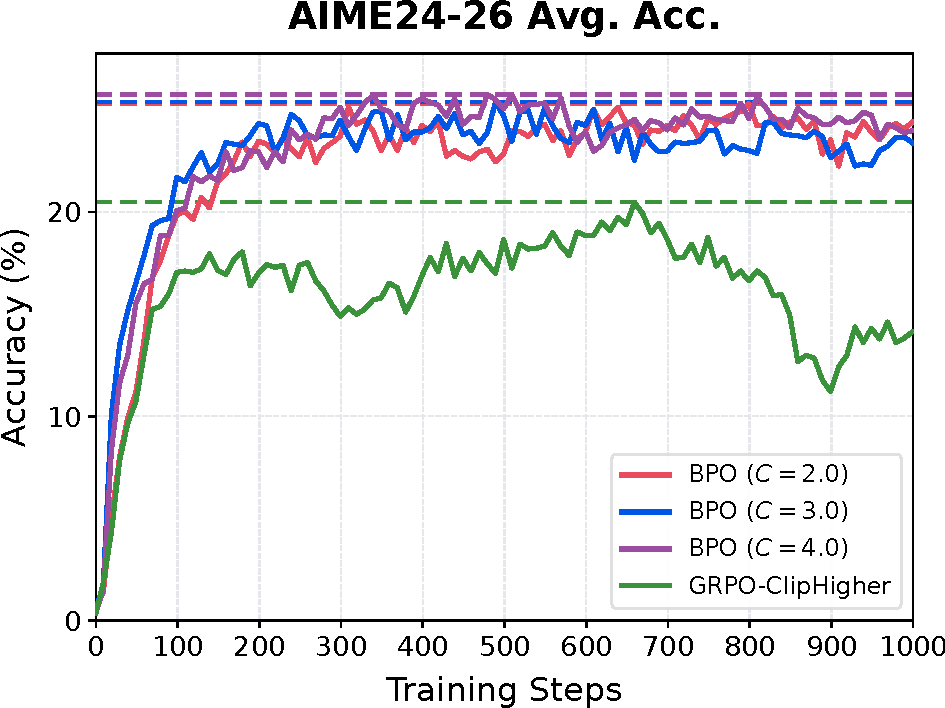
\includegraphics[width=0.8\linewidth]{figure/ab_bpo_4b_C_aime_avg.pdf}
\caption{BPO截断参数 $C$ 对 Qwen3-4B-Base 的影响，其中 $\epsilon=0.1$。曲线展示了 AIME24--26 上平均 Avg@32 的结果。虚线标记了每条曲线的峰值。}
\label{fig:capablation}
\end{figure}

\begin{table}[htbp]
\centering
\caption{BPO 截断参数 $C$ 的消融实验，使用 $\epsilon=0.1$，报告 AIME Avg@32 (\%)。每一行报告在三个基准上平均准确率最高的检查点的得分。每列中最佳结果以粗体标出。}
\label{tab:capablation}
\small
\renewcommand{\arraystretch}{1.1}
\begin{tabular}{lrrrr}
\hline
Method & AIME24 & AIME25 & AIME26 & Avg. \\
\hline
BPO ($C=2.0$) & 26.4 & 26.0 & \textbf{23.5} & 25.3 \\
BPO ($C=3.0$) & \textbf{27.6} & 26.8 & 21.8 & 25.4 \\
BPO ($C=4.0$) & 27.1 & \textbf{29.0} & 21.3 & \textbf{25.8} \\
GRPO-ClipHigher & 22.1 & 22.8 & 16.6 & 20.5 \\
\hline
\end{tabular}
\end{table}

$C$ 的三个取值产生的平均准确率在 25.3\% 到 25.8\% 之间，相差 0.5 个百分点。这三个结果均超过 GRPO-ClipHigher 基准的 20.5\%。这些结果表明，BPO 对 $C$ 从 $2.0$ 到 $4.0$ 的变化不敏感。

\end{appendices}

\end{document} 
